% Created 2021-02-23 mar. 09:19
% Intended LaTeX compiler: pdflatex
\documentclass[11pt]{article}
\usepackage[utf8]{inputenc}
\usepackage[T1]{fontenc}
\usepackage{graphicx}
\usepackage{grffile}
\usepackage{longtable}
\usepackage{wrapfig}
\usepackage{rotating}
\usepackage[normalem]{ulem}
\usepackage{amsmath}
\usepackage{textcomp}
\usepackage{amssymb}
\usepackage{capt-of}
\usepackage{hyperref}
\author{Victor Trappler}
\date{\today}
\title{}
\hypersetup{
 pdfauthor={Victor Trappler},
 pdftitle={},
 pdfkeywords={},
 pdfsubject={},
 pdfcreator={Emacs 26.3 (Org mode 9.1.9)}, 
 pdflang={English}}
\begin{document}

\begin{verbatim}
import numpy as np
import matplotlib.pyplot as plt
import seaborn as sns

x = np.arange(10)
y = x + np.random.normal(size=10)
plt.plot(x, y)
plt.savefig('../images/test_python.png')
return '../images/test_python.png' 
\end{verbatim}
And make sure to toggle the display of inline images \texttt{C-c C-x C-v}.
\begin{center}
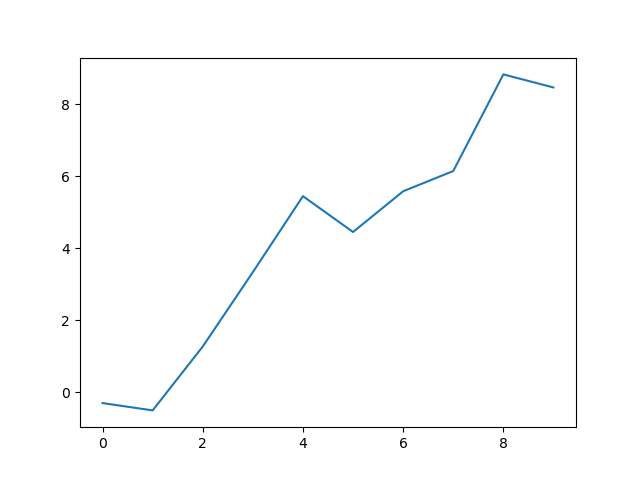
\includegraphics[width=.9\linewidth]{../images/test_python.png}
\end{center}
\end{document}